\documentclass[a4paper, 10pt, final, garamond]{book}
\usepackage{cours-preambule}

\makeatletter
\renewcommand{\@chapapp}{Devoir surveill\'e -- num\'ero}
\makeatother

\begin{document}
\setcounter{chapter}{5}

\chapter{Commentaires sur le DS n\degree06}

\section{Commentaires généraux}

Les outils d'énergétique ne sont pas acquis. Moyenne à 09/20. Il faut absolument
savoir déterminer une énergie potentielle à partir d'une force. Retravaillez
cette méthode, elle sera présente au prochain DS~: il suffit de partir de
\[
	\delta W(\Ff\ind{cons}) = \Ff\ind{cons}\cdot \dd{\OM} = -\dd{\Ec_p}
\]
et d'exprimer $\delta W(\Ff\ind{cons})$ comme l'opposé d'une différentielle.
\smallbreak
\textbf{Attention}, les énergies potentielles s'expriment \textbf{avec une
	constante}~! Trop souvent oubliée. Elles peuvent donc être négatives sans
aucun souci.
\smallbreak
\begin{center}
	\large Il ne faut pas dire «~référentiel\ftn{Et «~référenciel~» c'est joli,
		mais c'est une faute d'orthographe, évitez…} supposé galiléen~» sans dire
	\textbf{lequel}~!
\end{center}

\begin{figure}[htbp!]
	\centering
	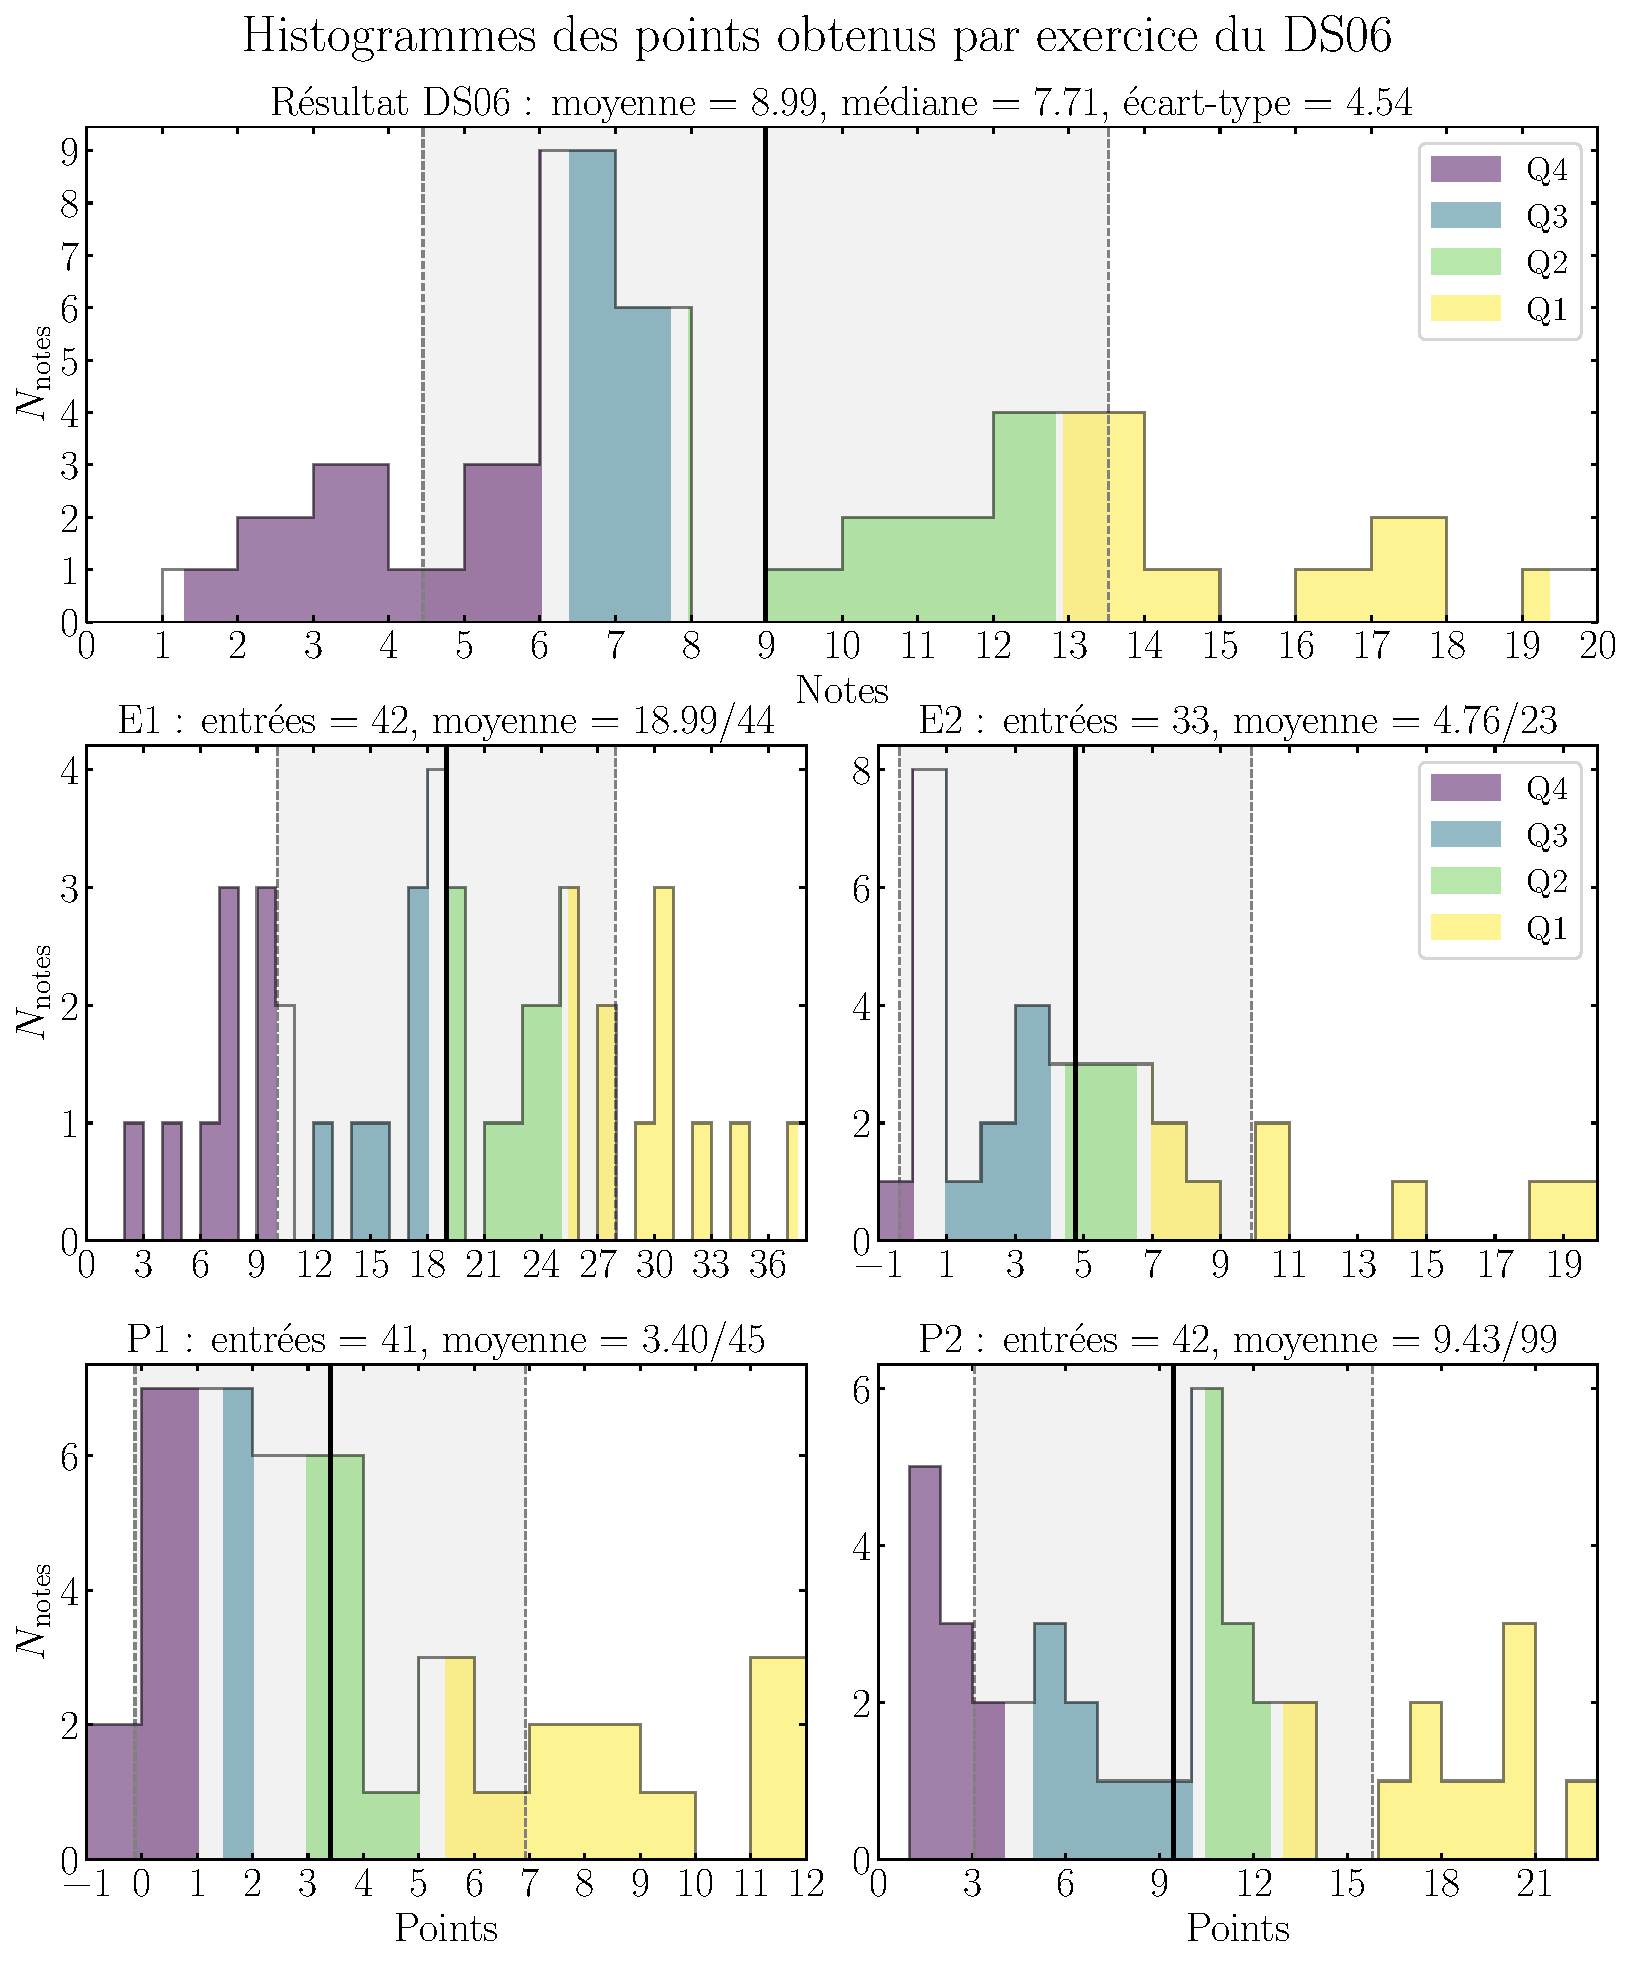
\includegraphics[width=.8\linewidth]{DS06_hist_all}
\end{figure}

\setcounter{section}{0}
\exercice[44]{Molécules de \textsc{Lewis}}
Un exercice très simple qui, comme annoncé, vaut beaucoup dans une copie. Il est
donc anormal d'avoir des schémas de \textsc{Lewis} qui ne respectent pas la
règle de l'octet et ce de manière ostentatoire, ou avec des hydrogènes qui font
3 liaisons. Malus «~O~» et «~D~» pour règle de l'octet/duet non respectée
(cumulables).
\smallbreak
Expliquez comment vous obtenez les charges formelles.
\smallbreak
Trop de confusion entre molécules, atomes, forces intermoléculaires ou
intramoléculaires… C'est anormal pour des apprentiz scientifiques de ne pas
savoir distinguer atome, particule, élément et molécule~!
\smallbreak
AM2 n'a pas \textbf{du tout} été compris. Soit vous pensez que les liaisons de
\textsc{VdW} sont répulsives (!!), soit qu'elles agissent au sein d'une molécule
(!!). Ce sont des forces \textbf{inter}moléculaires, donc \textbf{entre}
molécules, et elles sont toutes \textbf{attractives} et assurent la cohésion des
ensembles de molécules~; d'où la compétition avec l'énergie thermique qui tend à
rompre les liaisons intermoléculaires.
% \begin{enumerate}
% 	\nitem{4}% Q1
% 	\nitem{1}% Q2
% 	RAS.
% 	\nitem{1}% Q3
% 	RAS.
% 	\nitem{2}% Q4
% 	RAS.
% 	\nitem{3}% Q5
% 	\nitem{2}% Q6
% 	\nitem{1}% Q7
% 	\nitem{7}% Q8
% 	\item \begin{enumerate}
% 		      \nitem{2}% Q9a
% 		      \nitem{2}% Q9b
% 		      \nitem{2}% Q9c
% 		      \nitem{2}% Q9d
% 	      \end{enumerate}
% 	\item \begin{enumerate}
% 		      \nitem{2}% Q10a
% 		      \nitem{3}% Q10b
% 		      \nitem{3}% Q10c
% 	      \end{enumerate}
% \end{enumerate}

\exercice[23]{Toboggans}
Particulièrement décevant. Vous vous reposez sur vos habitudes et non sur les
définitions et sur l'établissement propre et rigoureux des résultats. C'était
censé être l'exercice facile qui donne 15 points à tout le monde…
\begin{enumerate}
	\nitem{2}% Q1
	Il faut comprendre le lien entre $z$ et $\th$…
	\nitem{2}% Q2
	Différentes manières de répondre. L'utilisation de $\delta W(\Pf)$ ou
	$W\ind{AB}(\Pf)$ est une bonne idée, mais il faut retenir que
	\[
		\delta W(\Pf) = \boxed{-}\dd{\Ec_p}
		\Lra
		W\ind{AB}(\Pf) = \boxed{-}\Delta\ind{AB}{\Ec_p}
	\]
	\nitem{5}% Q3
	Mauvaise détermination des énergies initiales et finales.
	\nitem{2}% Q4
	Coordonnées cylindriques = \textbf{polaire + $z$}~!!
	\nitem{2}% Q5
	RAS.
	\nitem{6}% Q6
	Attention aux variables utilisées pour les dérivées~: pour le TPM, on dérive
	$\Ec_m$ par rapport au \textbf{temps}, pas à l'angle~!
	\begin{center}
		\fbox{\textbf{Ce qui se conserve c'est dans le temps, ce qui évolue c'est
				dans l'espace}}
	\end{center}
	\nitem{3}% Q7
	Bien quand traitée.
\end{enumerate}

\setcounter{section}{0}
\prblm[45]{Haut-parleur électrostatique}
\begin{enumerate}
	\nitem{2}% Q1
	Il ne faut pas oublier les bases des chapitres de début d'année.
	\nitem{3}% Q2
	\textbf{Personne} n'a compris qu'un solide de charge $q = -Q$ subit la force
	$\Ff_e = -Q\Ef$…
	\nitem{2}% Q3
	Il vaut mieux donner la relation $\delta W(\Ff) = -\dd{\Ec_p}$, puisque
	l'expression du gradient n'est pas donnée.
	\nitem{6}% Q4
	$\Ef$ dépend de $z$…
	\nitem{3}% Q5
	Précisez quelles sont les forces qui sont conservatives.
	\nitem{2}% Q6
	RAS.
	\nitem{3}% Q7
	RAS.
	\nitem{3}% Q8
	RAS.
	\nitem{6}% Q9
	Globalement bien~! N'hésitez pas à tracer des fonctions sur votre calculatrice
	pour comprendre le phénomène/confirmer vos résultats. Par contre, évitez de
	développer tous les polynômes que vous avez, il faut mieux maîtriser le calcul
	et ne pas se ramener à des calculs machinaux à base de discriminant quand les
	racines sont évidentes.
	\nitem{1}% Q10
	RAS.
	\nitem{4}% Q11
	Très peu traitée.
	\nitem{3}% Q12
	Attention au signe de $z_0$.
	\nitem{4}% Q13
	Typique question de cours.
	\nitem{3}% Q14
	RAS.
\end{enumerate}

\prblm[99]{Lentillage magnétique}
\textbf{$\Bf$ et $\Ef$ ne sont pas des forces~!!}
\begin{enumerate}
	\nitem{3}% Q1
	Ne pas confondre réfraction et diffraction.
	\nitem{5}% Q2
	Analogie entre $\gf$ et $\Ef$ pour savoir dans quel sens il varie~: hauts
	potentiels vers bas potentiels. Ne pas sauter sur le sens de $\Ef$ pour dire
	que $\Ff_e$ est dans le même sens~: dépend de la charge du système~!
	\nitem{6}% Q3
	Déterminer $=$ démontrer.
	\nitem{8}% Q4
	Trop ratée. C'était gratuit comme points… attention à la définition de $U$ et
	au signe de $q = -e$.
	\nitem{2}% Q5
	Bien.
	\nitem{6}% Q6
	N'inventez pas des directions de champ magnétique ou de vitesse initiale~!
	\begin{center}
		\textbf{Uniforme $\Lra$ vitesse constante en \xul{norme} !}
	\end{center}
	\nitem{5}% Q7
	Revoir le traitement des mouvements circulaires uniformes en coordonnées
	polaires. Schémas peu réalistes.
	\nitem{3}% Q8
	Souvent traité en cartésiennes. Il n'y a pas que la méthode du cours qui
	existe. En TD on a répété ce résultat avec 2 autres méthodes, base de
	\textsc{Frenet} et base polaire.
	\nitem{3}% Q9
	Relativement bien.
	\nitem{5}% Q10
	Trop peu traitée.
	\nitem{4}% Q11
	Bien quand traitée.
	\smallbreak
	RAS sur le reste.
\end{enumerate}

\end{document}
